\chapter{Auswertung}
\label{auswertung}
Im Rahmen dieses Abschnitts werden die verschiedenen Phänomene und Aspekte, die bereits bei der Betrachtung und Interpretation der Ergebnisse der Messreihe angesprochen werden, nochmals aufgegriffen und isoliert betrachtet. Dabei werden hauptsächlich die Durchsatzergebnisse herangezogen, da der Fokus bei der Besprechung der Messreihen in \autoref{ergebnisse} bereits hauptsächlich auf die Latenzwerte gelegt wird. So werden auch die Durchsatzangaben nochmals genauer aufgegriffen. Außerdem wird in \autoref{ergebnisse} bereits die Beobachtung gemacht, dass Latenz- und Durchsatzwerte beide ähnliche Ergebnisse aufweisen. Ist bei einer Messung der Durchsatz hoch weist diese auch eine niedrige Latenz auf und umgekehrt.

\section{Einordnung der Performance}
\label{auswertung:einordnung}
Bei der Beurteilung der Performance der Datenbanksysteme handelt es sich bei den im Rahmen der Arbeit erzielten Messergebnissen um eine einfache Aufgabe. So weist bei jeder Messreihe Neo4j den niedrigsten Latenz- und Durchsatzwert auf, gefolgt von Db2 Graph Beta 3 -- sollte es Teil der Messreihe sein -- und Db2 Graph V11.5.6.0. 

Bei der Betrachtung der in der Messreihe beschriebenen Ergebnisse fällt zugleich auf, dass es sich hierbei nicht um einen kleinen Unterschied zwischen den jeweiligen Datenbanksystemen handelt. So scheinen sich die Datenbanksysteme sowohl bei der durchschnittlichen Latenz als auch beim Durchsatz um einen ähnlichen Faktor zu unterscheiden. Um die Datenbanksysteme bezüglich ihrer Performance einordnen zu können, wäre ein solcher Performance-Faktor ein passendes Maß. 

Um eine dementsprechende Kennzahl zur Einordnung der Datenbanksysteme bezüglich ihrer Performance bereitstellen zu können, wird daher ein gemeinsamer Durchschnittswert für den Durchsatz der Operationen:
\begin{itemize}
    \item \texttt{getNode}
    \item \texttt{getLink}
    \item \texttt{countLink} und 
    \item \texttt{getLinkList} (Range-Limit 100) ermittelt.
\end{itemize}
Der gemeinsame Durchschnittswert für den Durchsatz wird dabei einmal für jedes Datenbanksystem im Kontext einer Messreihe ermittelt. Anschließend wird der niedrigste Wert einer Messreihe herangezogen -- immer Db2 Graph V11.5.6.0 -- und als Faktor eins festgelegt. Im nächsten Schritt werden basierend auf diesem Faktor eins und seinem Durchschnittswert die jeweiligen Faktoren für Neo4j und gegebenenfalls Db2 Graph Beta 3 errechnet. Die dabei erhaltenen Performance-Faktoren -- basierend auf dem Durchsatz -- werden für die Messreihen mit einem konstant-verteilten Datensatz in \autoref{fig:faktor:durchsatz:const} dargelegt, während die mit real-verteilten Datensätzen in \autoref{fig:faktor:durchsatz:real} abgebildet werden.

\begin{figure}[!ht]
    \centering
    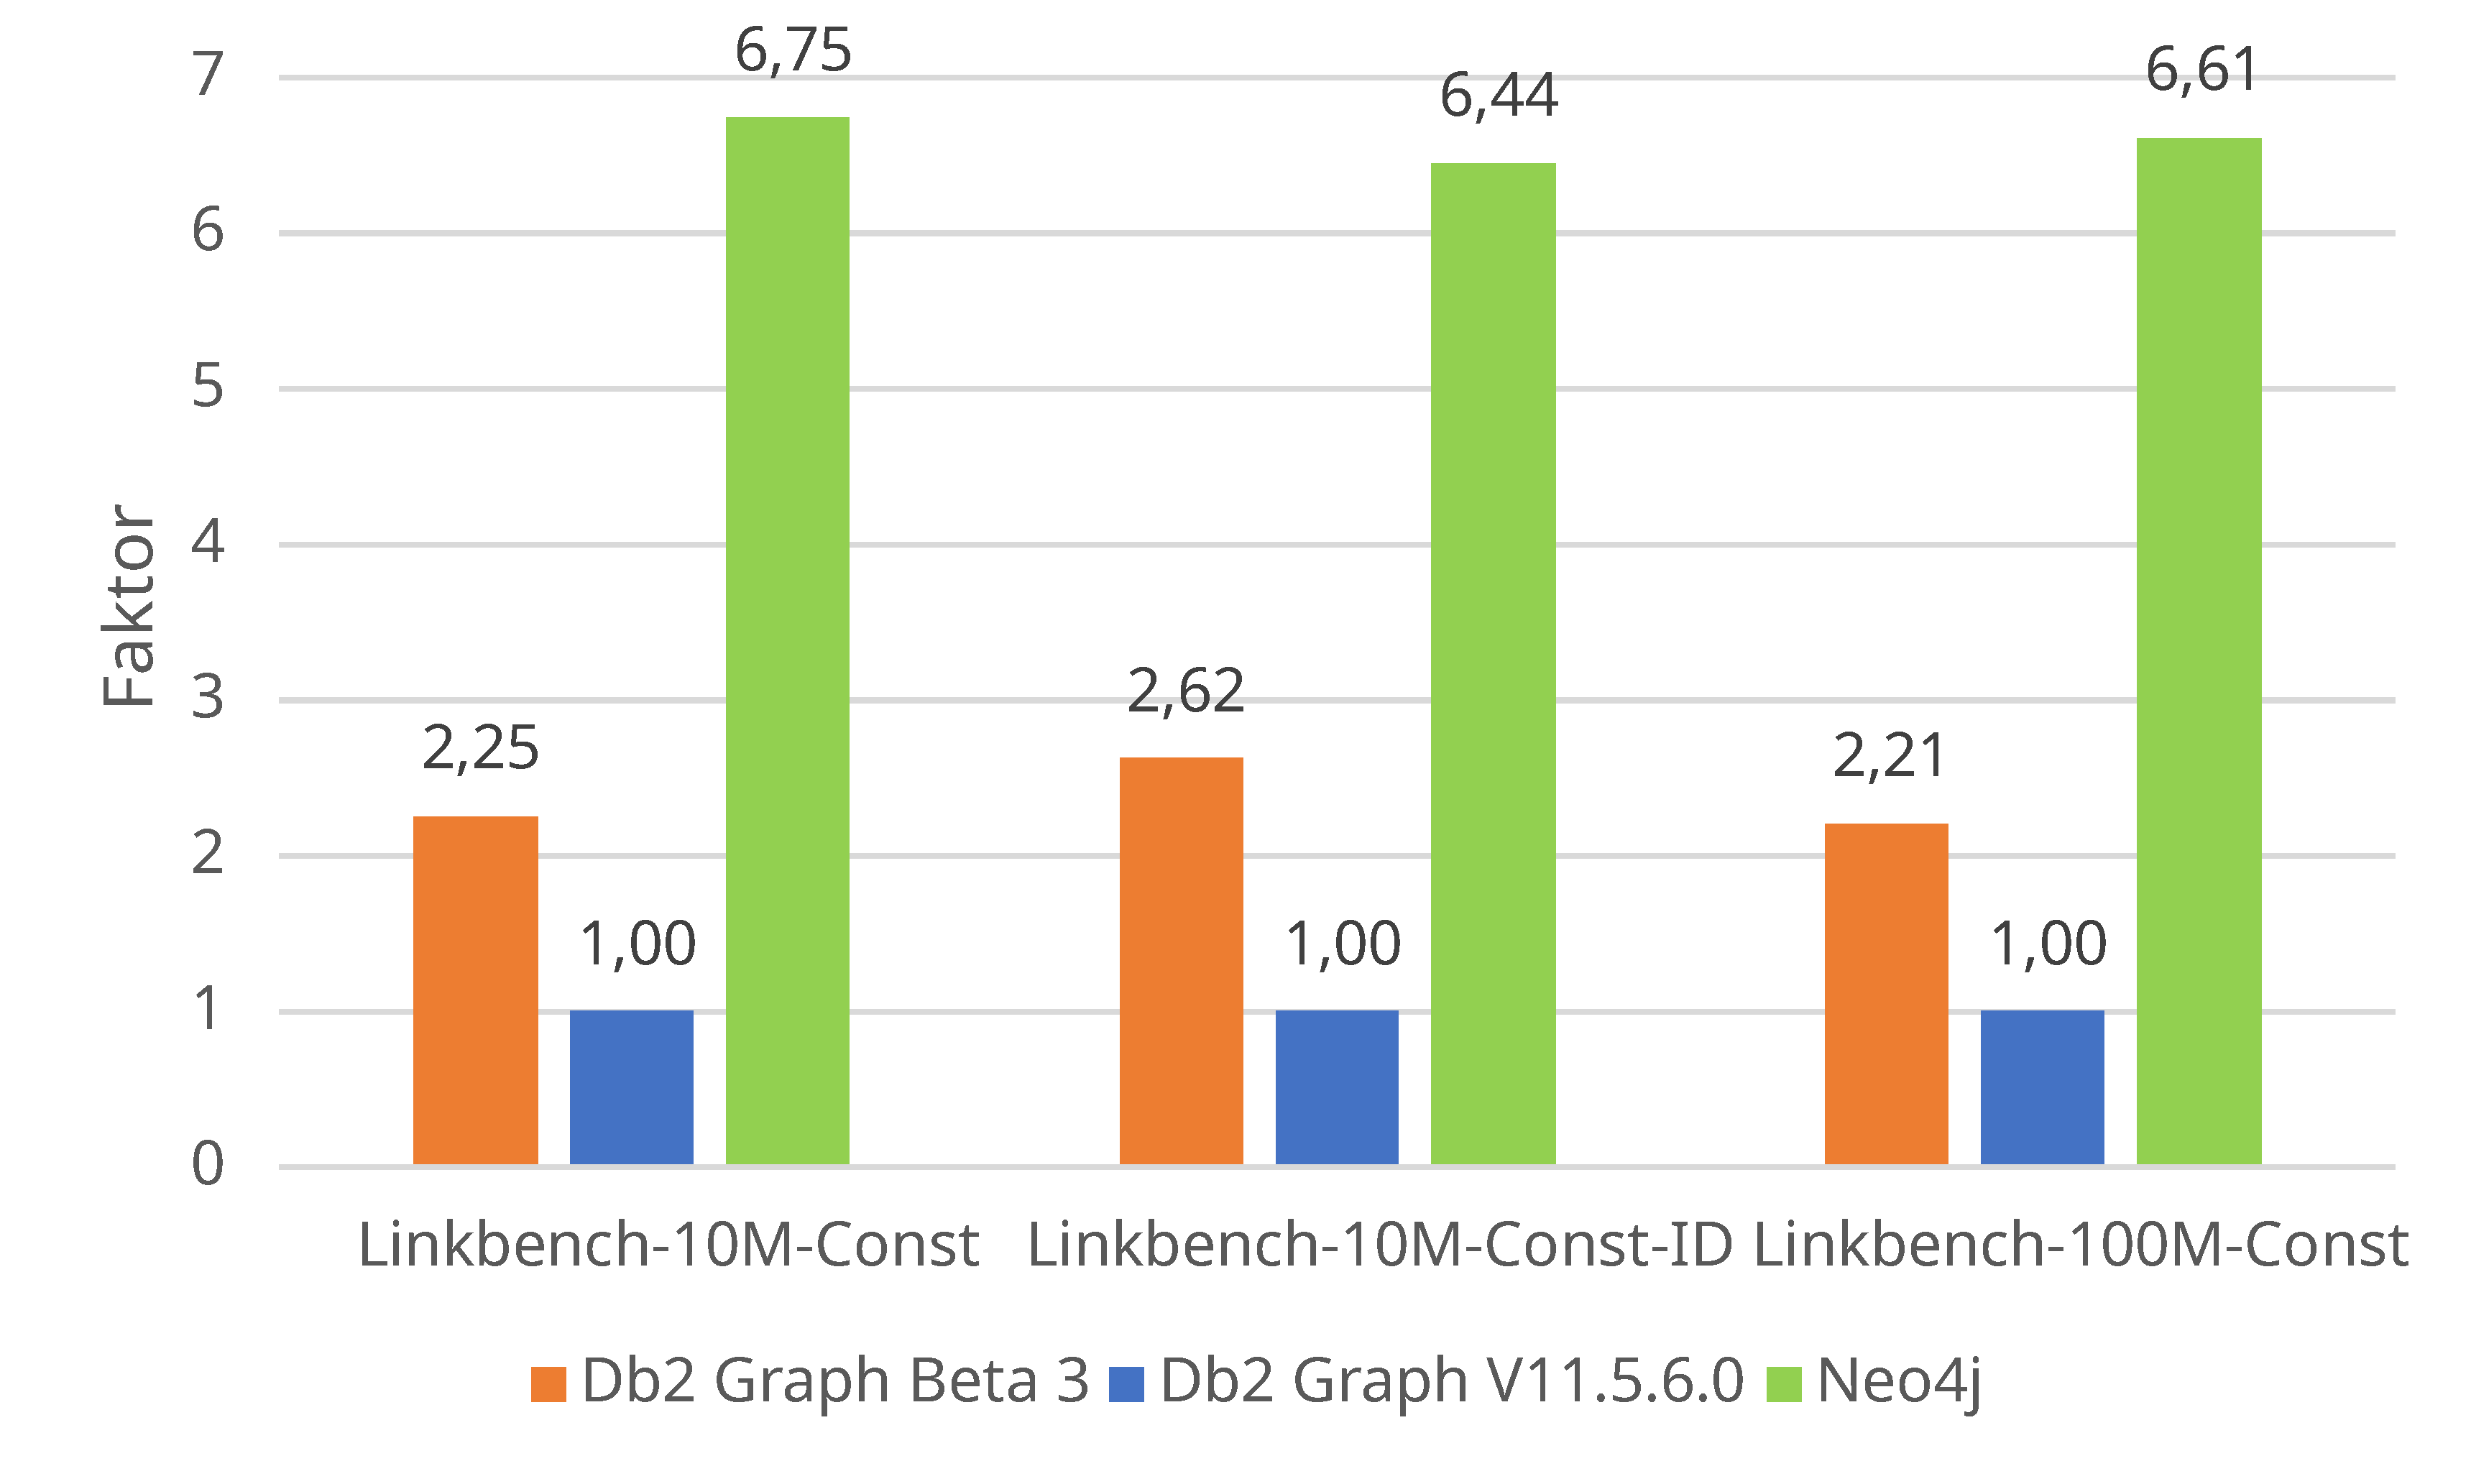
\includegraphics[width=\textwidth]{images/diagramme/faktor_durchschittlicher_durchsatz_const.pdf}
    \caption{Performance-Faktor bei Messreihen mit konstant-verteilten Datensätzen}
    \label{fig:faktor:durchsatz:const}
\end{figure}

\begin{figure}[!ht]
    \centering
    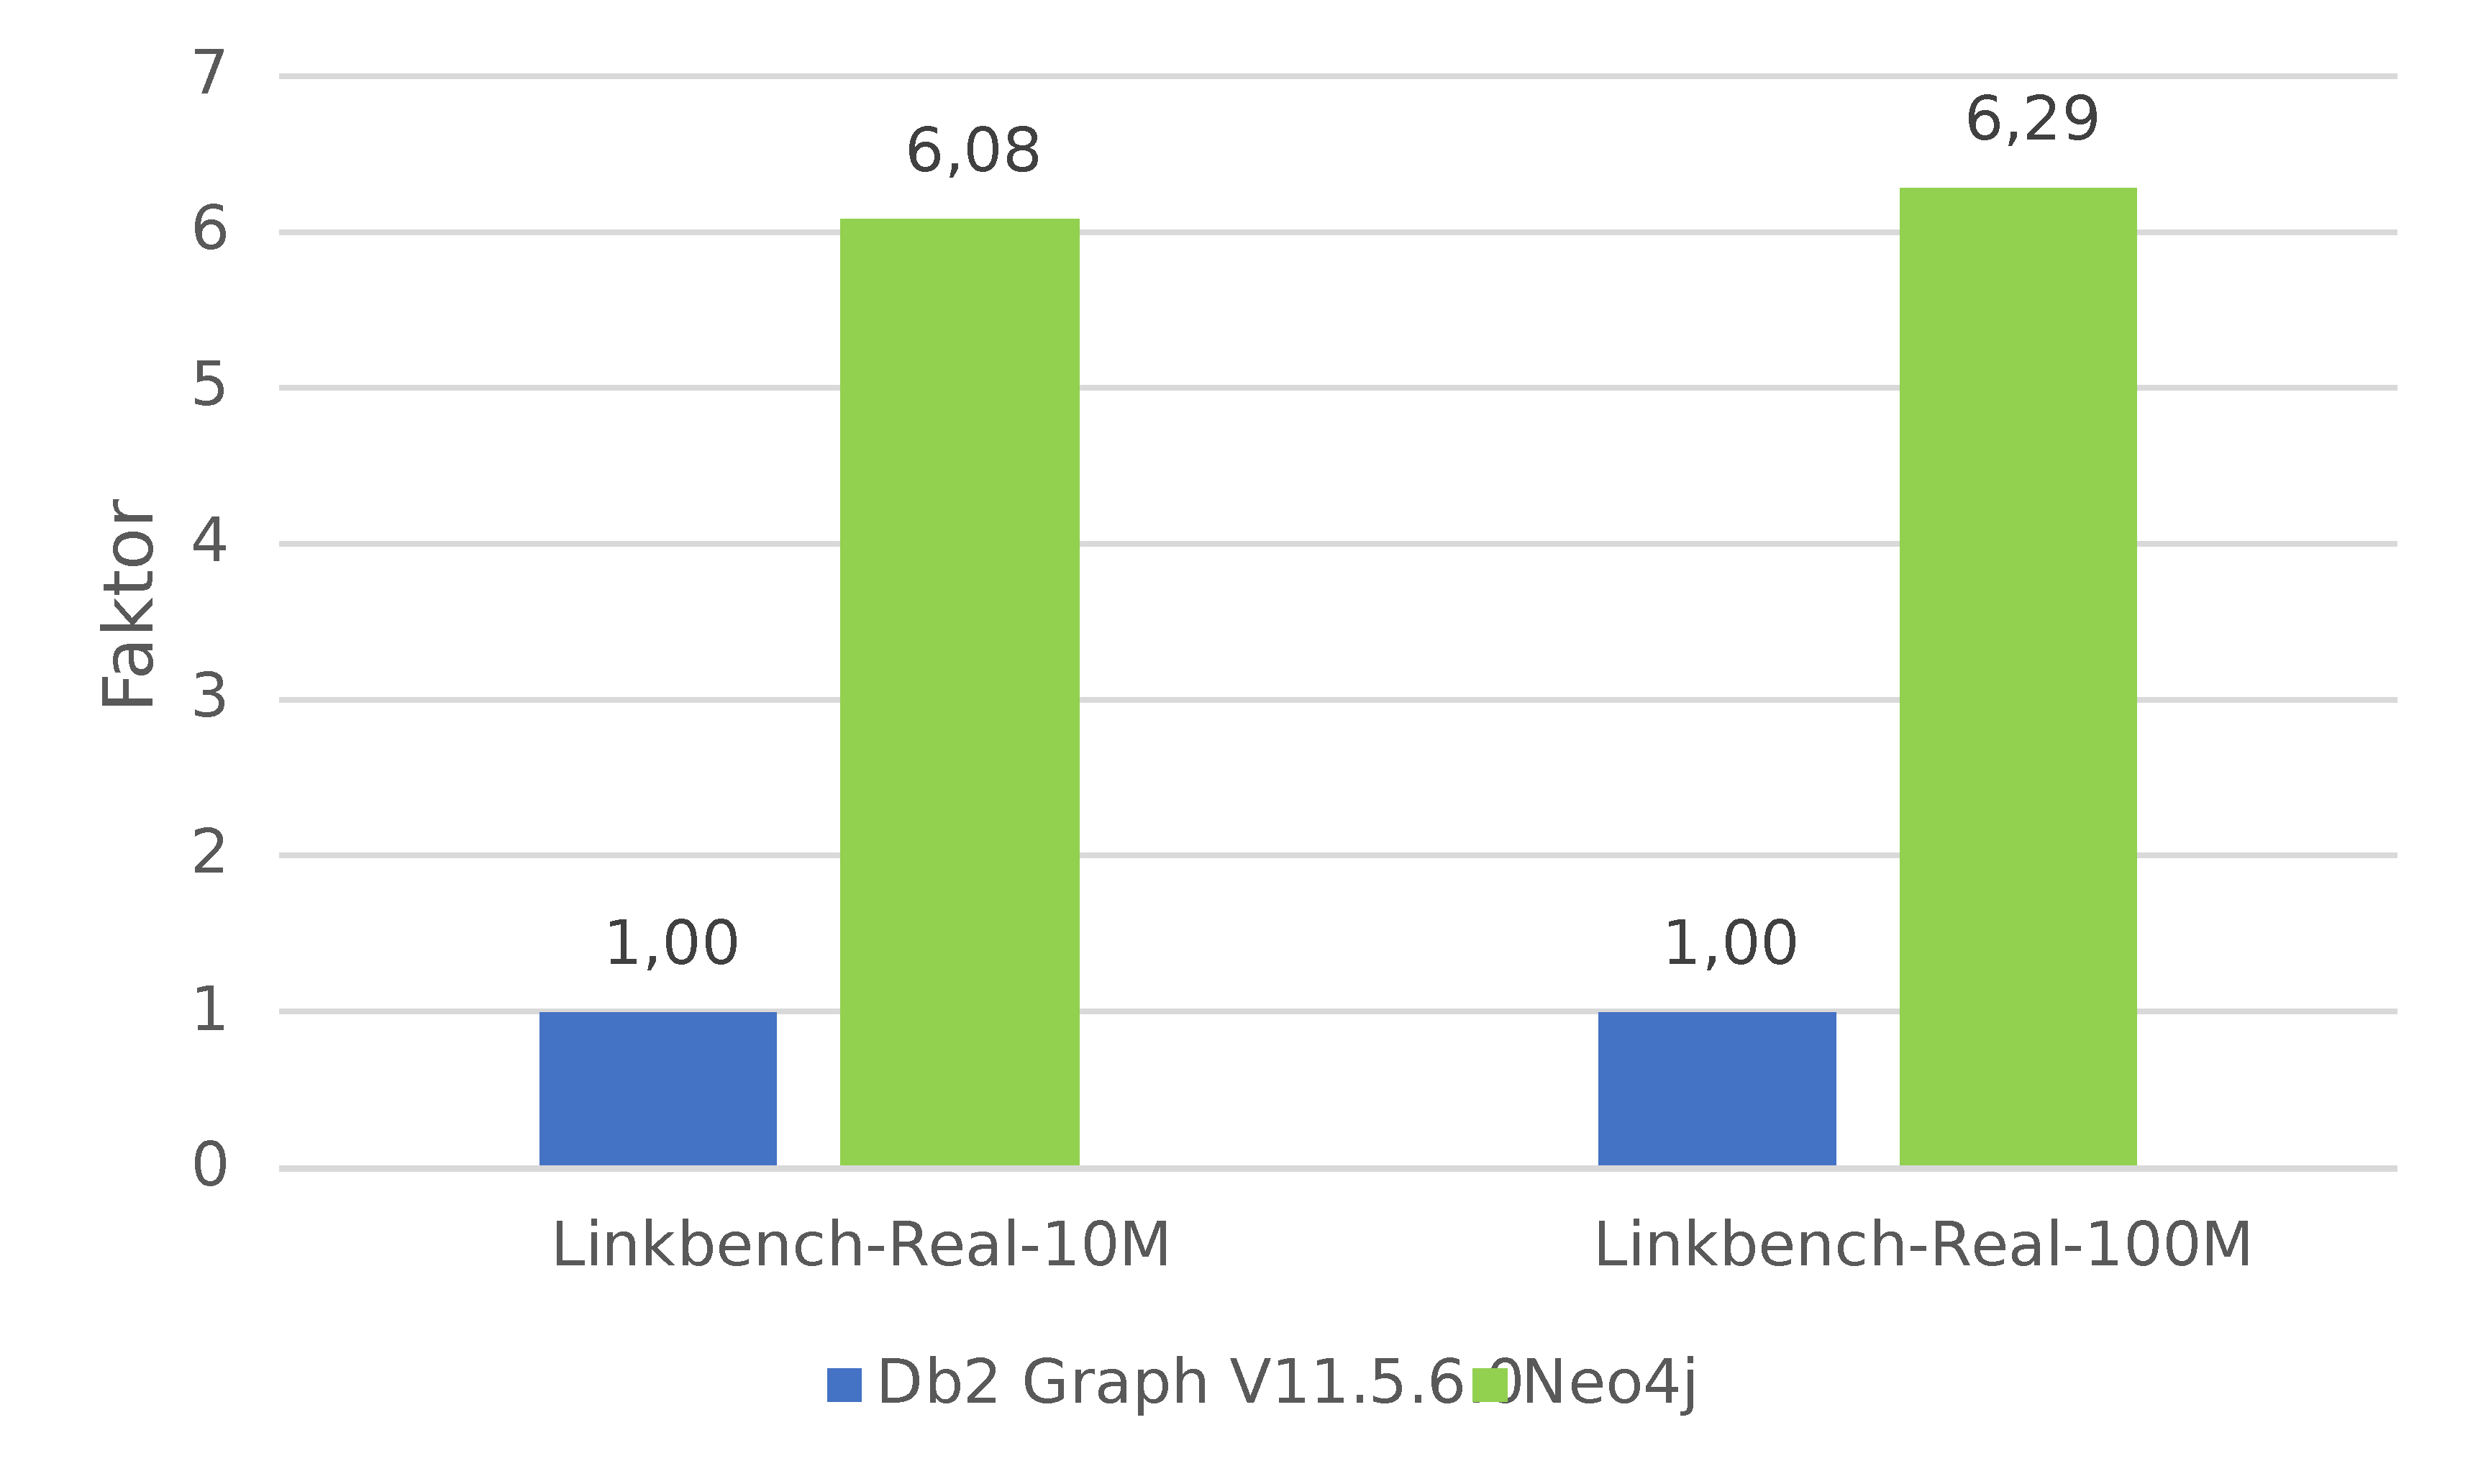
\includegraphics[width=\textwidth]{images/diagramme/faktor_durchschittlicher_durchsatz_real.pdf}
    \caption{Performance-Faktor bei Messreihen mit real-verteilten Datensätzen}
    \label{fig:faktor:durchsatz:real}
\end{figure}

Bei der Analyse der in \autoref{fig:faktor:durchsatz:const} und \autoref{fig:faktor:durchsatz:real} dargestellten Faktoren fällt auf, dass Neo4j immer 6- bis 7-Mal so viele Operationen pro Sekunde bearbeitet wie Db2 Graph bei den jeweiligen Messreihen, was einen gewaltigen Performance-Unterschied zwischen Db2 Graph V11.5.6.0 offenbart. Der Performance-Unterschied zwischen Db2 Graph Beta 3 und Neo4j um ein zwei- bis dreifaches bei den Faktoren in \autoref{fig:faktor:durchsatz:const} ist hier etwas geringer.

So war anfänglich nicht davon auszugehen das Db2 Graph als Grapherweiterung in Kombination mit Db2 Neo4j als natives Graphdatenbanksystem übertrifft. Schließlich verursacht die Kommunikation zwischen Db2 Graph und Db2, die für die Beantwortung einer Anfrage nötig ist, einen Aufwand den Neo4j nicht betreiben muss. Einen Performance-Unterschied um mindestens den Faktor 6 galt es jedoch nicht zu erwarten. 

Eine interessante Gegebenheit, die in der \autoref{fig:faktor:durchsatz:const} beobachtet werden, kann stellt der Fakt dar, dass Db2 Graph Beta 3 als ältere Version von Db2 Graph 2 bis 2,5 Mal mehr Operationen pro Sekunde bewältigen kann, als Db2 Graph V11.5.6.0 (der erste GA Release). Zu Beginn wäre hier eigentlich die Vermutung nahe gelegen, dass V11.5.6.0 als neuere Version, die über mehr Optimierungstechniken verfügt als Beta 3, eine höhere Performance aufweist. Dies ist allerdings nicht der Fall. 

Dabei gilt es hingegen zu beachten, dass Db2 Graph Beta 3 trotz der höheren Performance bei den Messreihen mit konstant-verteilten Datensätzen nicht als allgemein performantere Version von Db2 Graph einzustufen ist. Schließlich spielt sie bei den Messreihen mit real-verteilten Datensätzen keine Rolle, da sie für den Einsatz dort aufgrund fehlender Optimierungstechniken derart ungeeignet ist, dass das Erzielen von Ergebnissen im Rahmen des üblichen Zeitraums nicht möglich ist.

\section{Umgang mit Ergebnismengen}
\label{auswertung:ergebnismenge}
Bei der Untersuchung der Ergebnismenge bei den Messreihen mit real-verteilten Datensätzen wird bereits in \autoref{ergebnisse:10m_real} und \autoref{ergebnisse:100m_real} ein kurzer Überblick über das jeweilige Verhalten bezüglich beim Durchsatzes gegeben. Wie große der verhältnismäßige Einbruch des Durchsatzes und entsprechend auch der Performance, bei einer variierenden oberen Grenze für die Anzahl an Elementen in einer Ergebnismenge ist, lässt sich an den Abbildungen, die absolute Zahlen präsentieren, nicht ablesen. Schließlich bewegen sich die Datenbanksysteme mit beispielsweise 15.742 und 2.466 Operationen pro Sekunde in \autoref{ergebnisse:10m_real} in anderen Größenordnung, werden aber in derselben Grafik abgebildet. 

Um nun der Frage auf den Grund zugehen: \textit{Welches Datenbanksystem bei einem steigenden Range-Limit den verhältnismäßig größeren Performance-Einbruch aufweist?}, wird in \autoref{fig:einbruch:durchsatz:10m} und \autoref{fig:einbruch:durchsatz:100m} dargestellt, wie viele Prozent des Durchsatzes bei einem steigenden Range-Limit noch erreicht werden können. Der Wert für \texttt{getLinkList} mit einem Range-Limit von 100 repräsentiert dabei jeweils 100 \% des Durchsatzes von Neo4j oder Db2 Graph. So sinkt beispielsweise der Durchsatz bei Neo4j in \autoref{fig:einbruch:durchsatz:10m} bei einem Range-Limit von 10.000 auf lediglich 69,74 \% des bei einem Range-Limit von 100 erzielten Durchsatzes. 

Bei der Betrachtung des Kurvenverlaufs in \autoref{fig:einbruch:durchsatz:10m} und \autoref{fig:einbruch:durchsatz:100m} fällt auf das der Durchsatz bei Neo4j eher linear aussieht, während Db2 Graph bei einem Range-Limit von 10.000 jeweils einen Knick aufweist. 

Des Weiteren ist erkennbar, dass der Performance-Einbruch bei Db2 Graph V11.5.6.0 bei einem steigenden Range-Limit immer geringer zu sein scheint, als bei Neo4j. So weist V11.5.6.0 bei einem Range-Limit von 100.000 noch 54,18 \% des Durchsatzes auf den es bei einem Range-Limit von 100 erreicht hat. Neo4j hingegen erlangt bei 100.000 lediglich 43,29 \% des Durchsatzes den es erreicht, wenn die Ergebnismenge auf eine obere Grenze von 100 Elemente begrenzt wird. 

So beträgt der Unterschied zwischen Db2 Graph und Neo4j bei einem Range-Limit von 100.000 ca. 11 \% zueinander in \autoref{fig:einbruch:durchsatz:10m}, während es bei 10.000 sogar ca. 18 \% sind. Bei einem Range-Limit von 1.000 sind es jedoch lediglich ca. 8 \% Unterschied zueinander. Wobei es bei hier anzumerken gilt, dass Db2 Graph mit 97,58 \% ein außergewöhnlich hohes Ergebnis erreicht. Die in \autoref{fig:einbruch:durchsatz:100m} dargestellten Werte bestätigen dabei grob die Beobachtungen aus \autoref{fig:einbruch:durchsatz:10m}. So weichen die Werte in den beiden Abbildungen (\autoref{fig:einbruch:durchsatz:10m} und \autoref{fig:einbruch:durchsatz:100m}) höchstens um bis zu 2 \% voneinander ab. 

\begin{figure}[!ht]
    \centering
    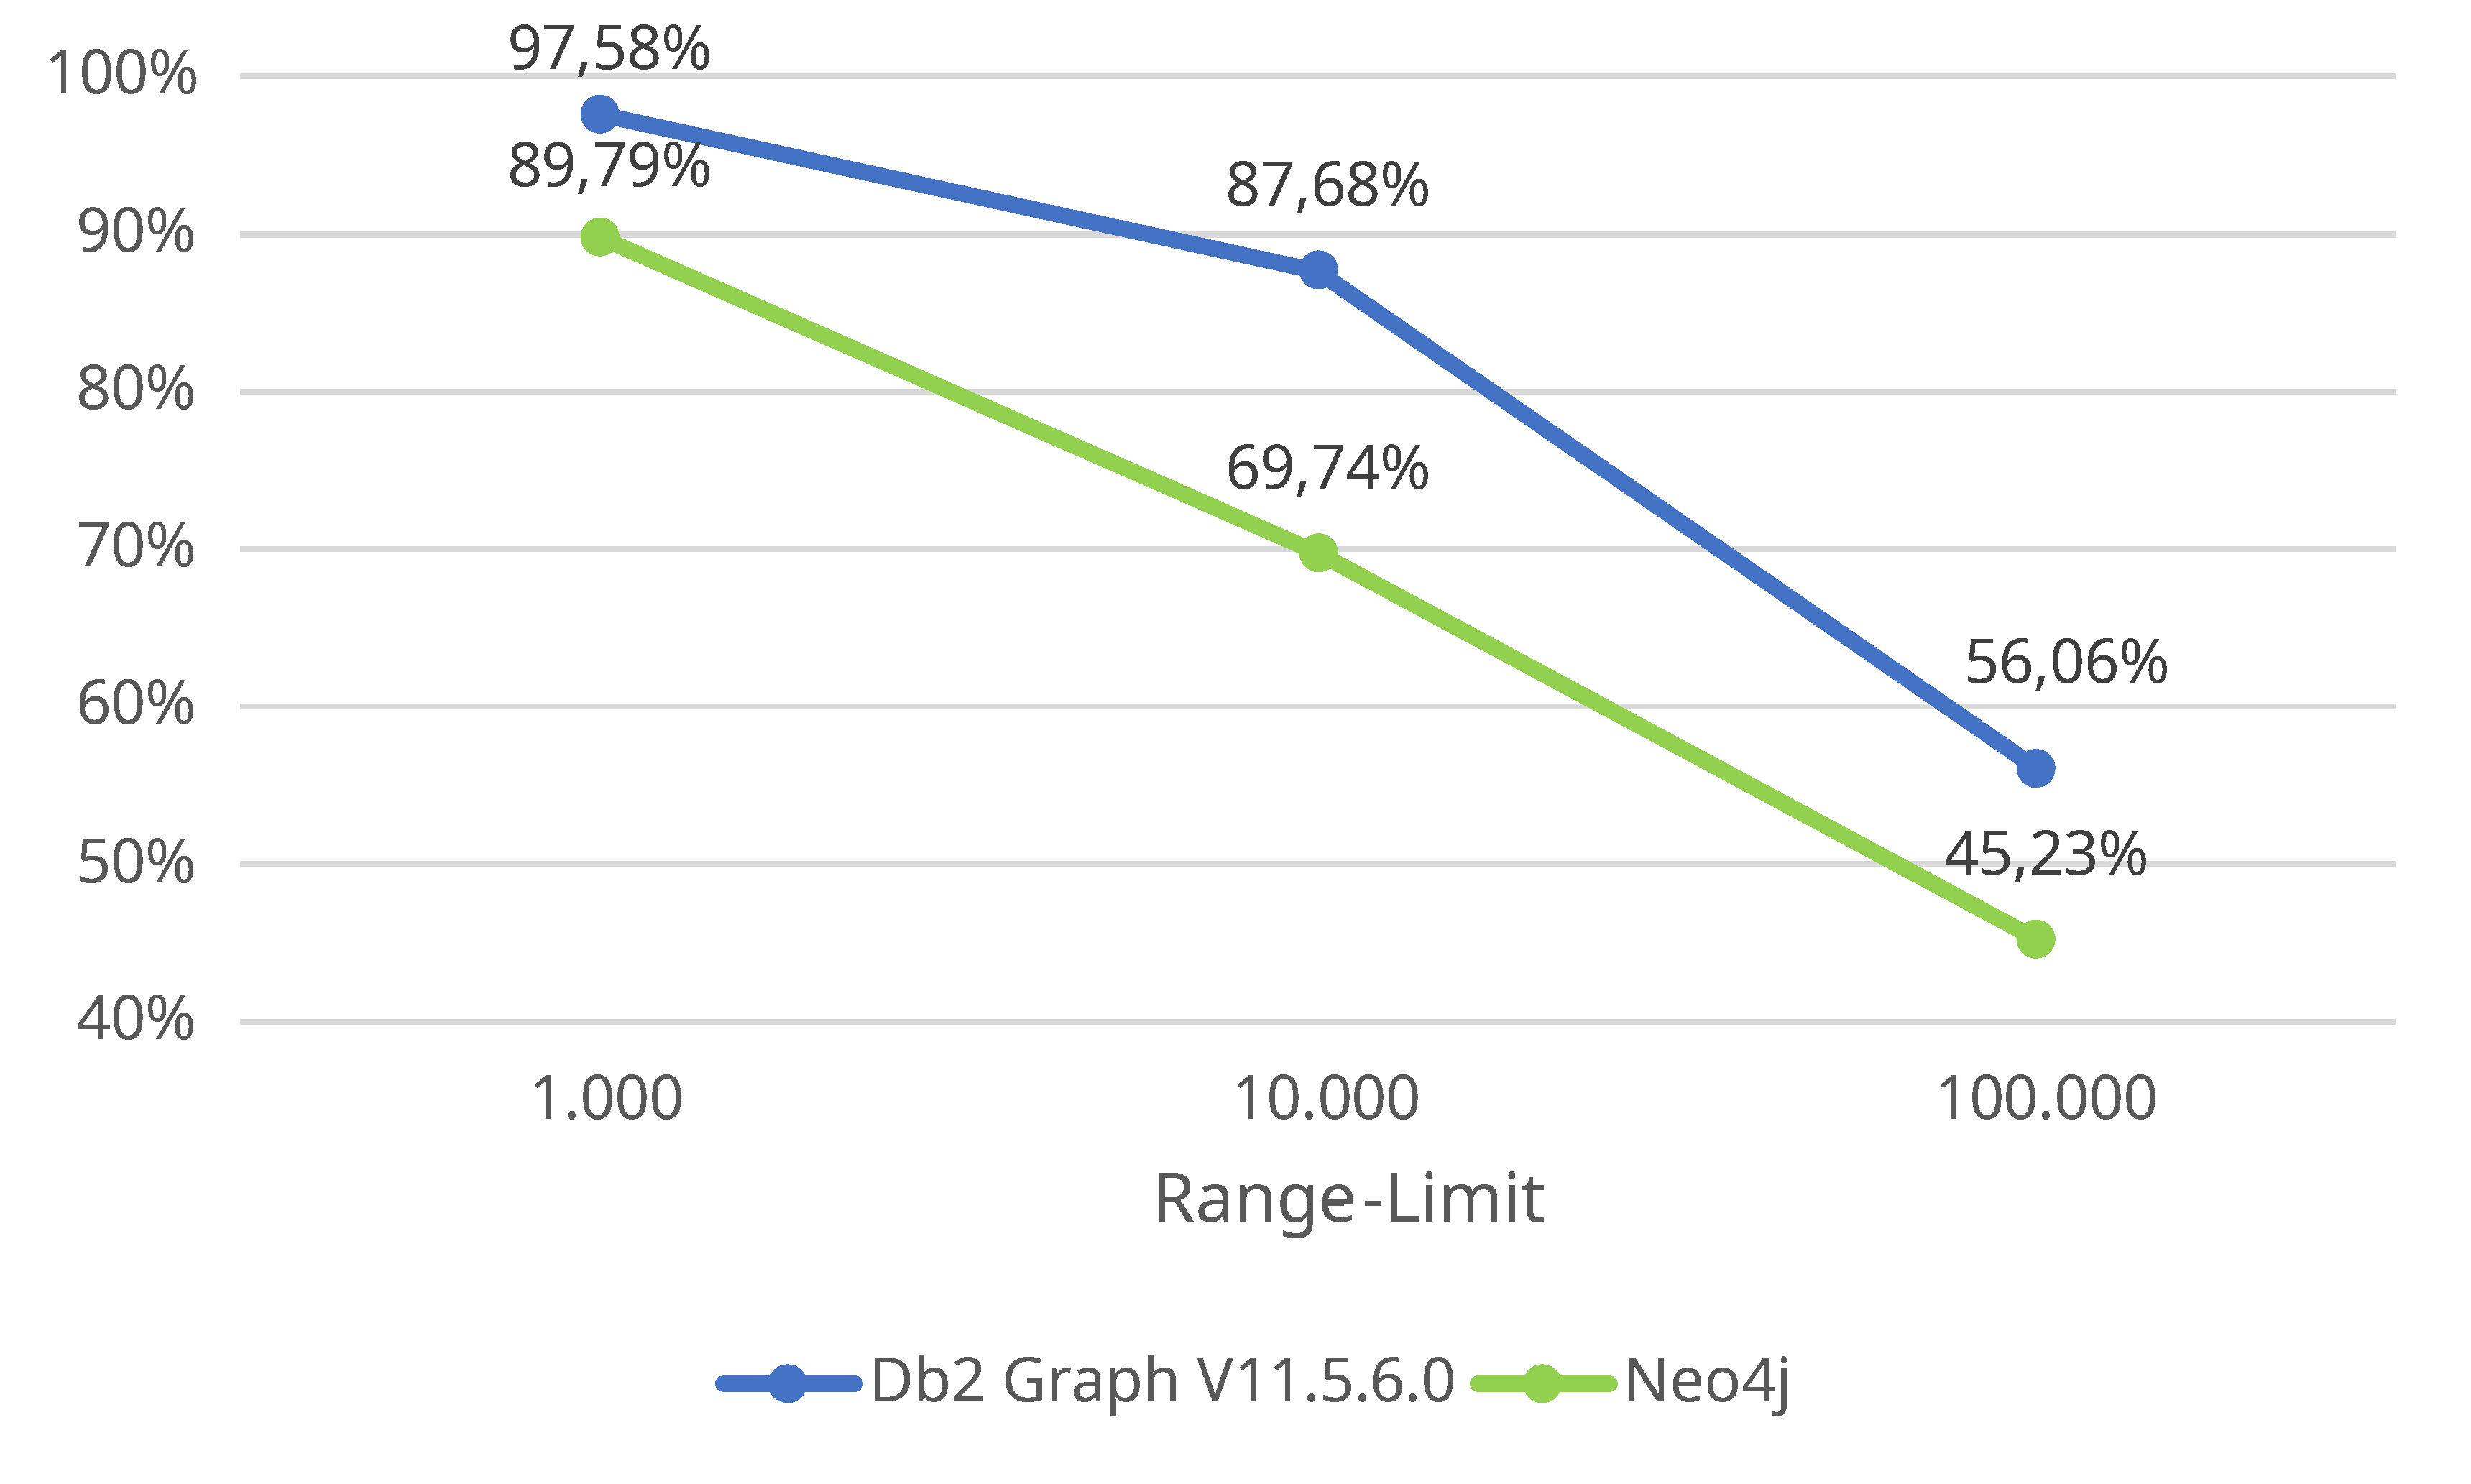
\includegraphics[width=\textwidth]{images/diagramme/limit_relative_durchsatz_real_10m.pdf}
    \caption{Linkbench-10M-Real Durchsatz gemessen an getLinkList(100)}
    \label{fig:einbruch:durchsatz:10m}
\end{figure}

\begin{figure}[!ht]
    \centering
    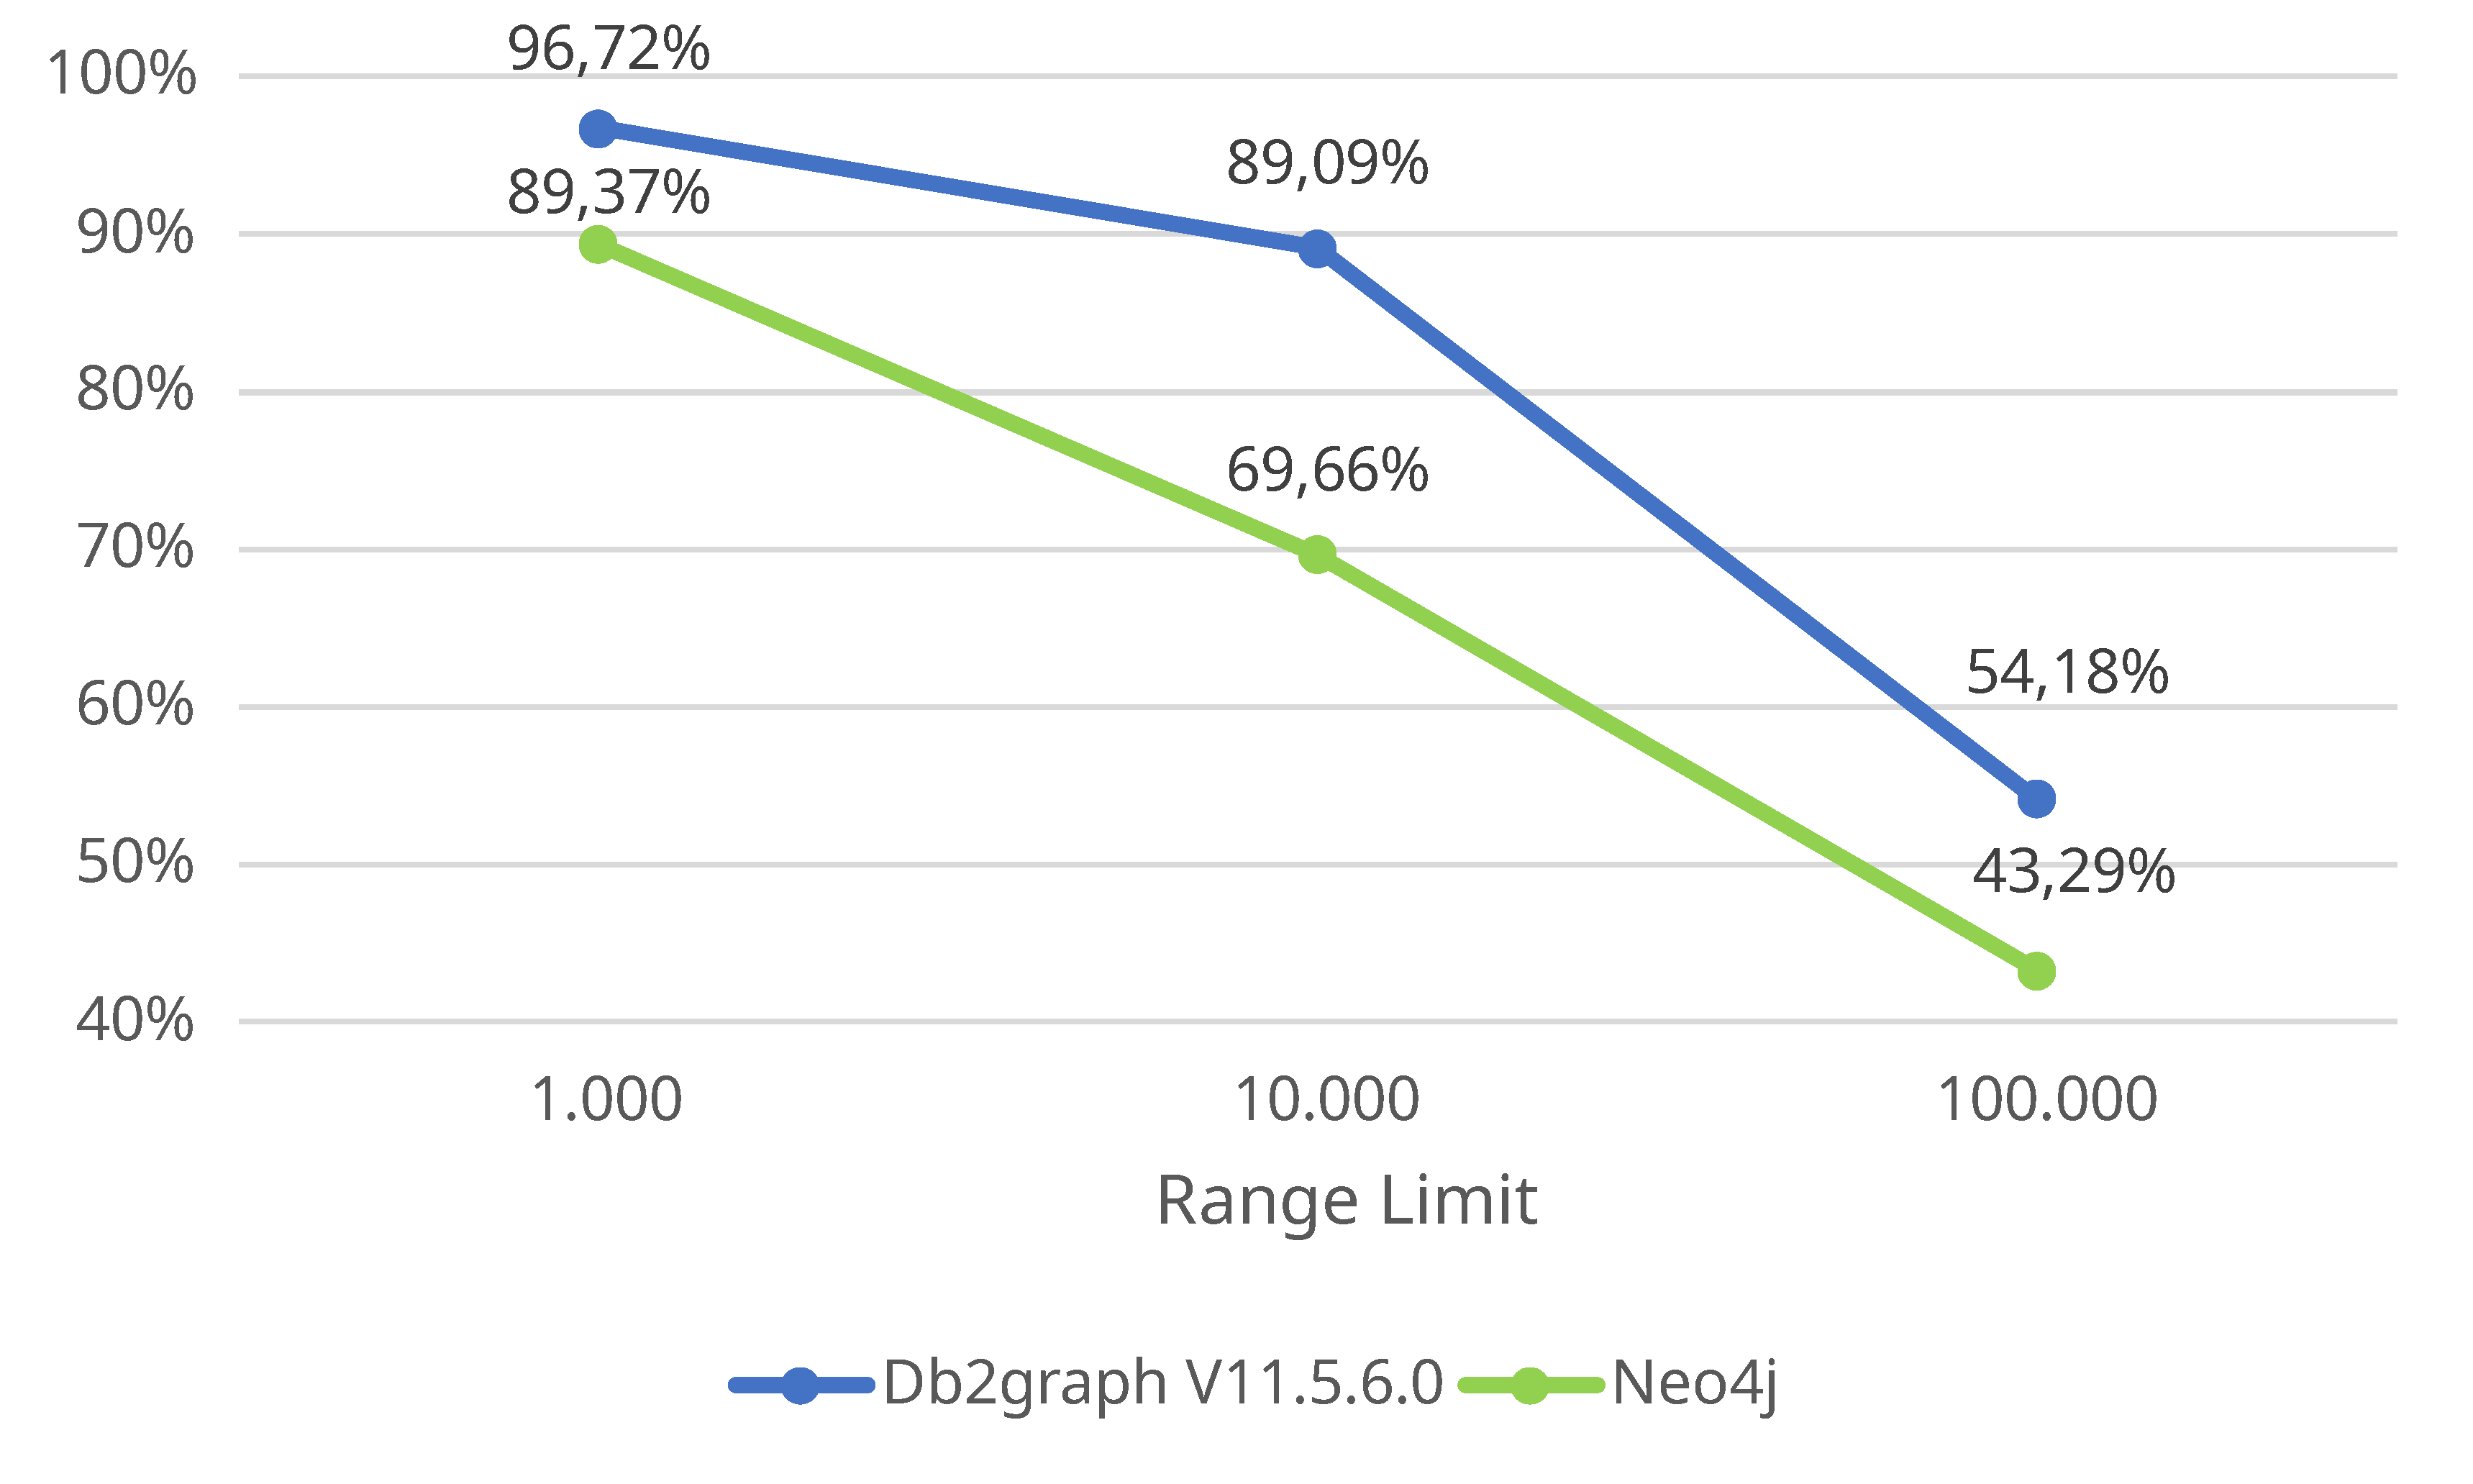
\includegraphics[width=\textwidth]{images/diagramme/limit_relative_durchsatz_real_100m.pdf}
    \caption{Linkbench-100M-Real Performance gemessen an getLinkList(100)}
    \label{fig:einbruch:durchsatz:100m}
\end{figure}

Schlussendlich kann basierend auf \autoref{fig:einbruch:durchsatz:10m} und \autoref{fig:einbruch:durchsatz:100m} das Fazit gezogen werden, dass der Performance Einbruch beim Umgang mit größeren Ergebnismengen bei Neo4j nicht nur in absoluten Zahlen ausfällt, sondern auch im Verhältnis.

\section{Einfluss der Datensatzgröße}
\label{auswertung:groesse}
Im Rahmen dieses Abschnitts wird genauer untersucht, wie groß d

\section{Vergleich zwischen den Verteilungen}
\label{auswertung:verteilung}

\section{Ressourcenauslastung}
\label{auswertung:ressourcenauslastung}

\todo{Auf Ressourcenauslastung verweisen.}

\listoftodos